% !TEX root = main.tex

\chapter{Existing experimental system}
In this chapter we are going to describe the essential parts of the already existing setup on top of which the addressing system has been built. Calcium-40 ions are used in the experiment, the implementation of several techniques for trapping and manipulating these ions are discussed. Furthermore, the addressing setup utilizes 393 nm light, the laser emitting this light was already installed by H. Hainzer\footnote{In her work, the 393 nm laser (MSquared Ti:Sa) and the ion cavity were locked to an ultrastable reference cavity. She measured the linewidth of the MSquared Ti:Sa laser to be <100 Hz with a drift rate of 202(1) mHz/s} \cite{helene}, thus that setup is briefly presented. The experiment can be controlled remotely via computers, an overview of how it is implemented and how it works is also given.

\section{Ion trap and key techniques}
\subsection{Calcium Ions}
\label{sec:calciumion}
\begin{figure}
\centering
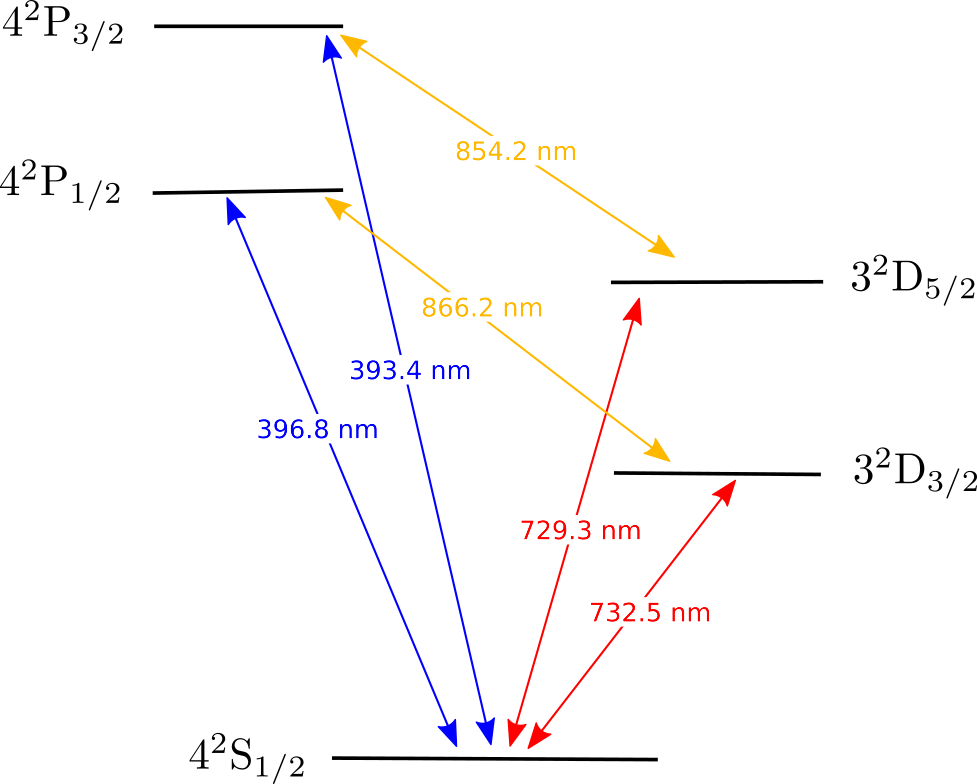
\includegraphics[width = .6 \textwidth]{calciumscheme}
\caption{Level scheme of $^{40}\text{Ca}^+$ with main transitions highlighted and Zeeman substructure. Blue transitions are dipole transitions suitable for cooling, imaging and photon detection. Red transitions are dipole forbidden, but accessible with electric quadrupole, they are used to encode qubits. Orange transition are usually repumped. In addition, the 854 nm transition is tuned in resonance with the cavity for photon generation purposes. From more and precise value see table \ref{transitiontable}}
\label{calciumscheme}
\end{figure}
For quantum computation purposes, ions with a single valence electron are an attractive choice, examples include beryllium \cite{beryllium}, barium \cite{barium}, strontium \cite{strontium}, calcium \cite{calcium}. Other trapped species include for example ytterbium \cite{PhysRevA.44.R20}, and magnesium \cite{magnesium}. In our experiment we trap $^{40}\text{Ca}^+$, the most abundant isotope of calcium. In figure \ref{calciumscheme} the level scheme of the valence electron is presented. We use the notation $n^{2s+1}l_j$, where $n$ is the principal quantum number, $s$ the electron spin, $l$ the orbital angular moment, and $j = |l\pm s|$ the total angular moment. In the experiment a magnetic field lifts the level degeneracy, thus the magnetic $m_j$ quantum number is also present. A ground state $\text{S}_{1/2}$ is present with no hyperfine structure as $^{40}\text{Ca}^+$ does not posses a nuclear spin. Two short lived excited states ($1/\Gamma \sim 7$ ns) $\text{P}_{1/2}$, and $\text{P}_{3/2}$ are connected to S via dipole transitions. These states have different decay channel, for $\text{P}_{1/2}$ the branching ratios are $6\%$ to $\text{D}_{3/2}$, and $94\%$ back to the ground state.
For $\text{P}_{3/2}$ there is a probability of $5.3\%$ to decay to $\text{D}_{5/2}$, $0.6\%$ to go to  $\text{D}_{3/2}$ and $94\%$ to return to  $\text{S}_{1/2}$. Due to the short lifetimes of these two states, they are suitable for laser cooling and state detection, while the states $\text{D}_{3/2}$ and $\text{D}_{5/2}$
are metastable ($ 1/\Gamma \sim 1$ s) and are coupled to the S state via electric quadrupole transition. An optical qubit can be implemented in the transition $\text{S}_{1/2} \to \text{D}_{5/2}$, as the lifetime of the $\text{D}_{5/2}$ state is longer than typical operation times \cite{calciumqubit}. Other choices for qubit implementation have been explored, for instance in the Zeeman levels of the $\text{S}_{1/2}$ manifold \cite{Ruster2016}. Table \ref{transitiontable} summarizes details about the different transitions, and what they are used for. A more detailed description and implementation is discussed in the next section.

\begin{table}[H]
\centering
\begin{tabular}{c c c c c}
 \toprule
    {Transition} & {wavelength (nm)} & {Decay rate $\Gamma$} & Lifetime $\tau$ & {Main use} \\ \midrule
   $\text{S}_{1/2} \to \text{P}_{1/2}$ & 396.847 & $2\pi \times 20.8$ MHz & 7.7 ns &  Cooling and imaging \\
    $\text{S}_{1/2} \to \text{P}_{3/2}$  & 393.366 & $2\pi \times 21.4$ MHz & 7.4 ns & Photon generation\\ \midrule
   $\text{S}_{1/2} \to \text{D}_{3/2}$ & 732.389 & $2\pi \times 0.132$ Hz & 1.080 s & - \\
    $\text{S}_{1/2} \to \text{D}_{5/2}$  & 729.147 & $2\pi \times 0.136$ Hz & 1.045 s   & Qubit  \\\midrule
    $\text{P}_{1/2} \to \text{D}_{3/2}$  & 866.214 &  $2\pi \times 1.70$ MHz  &  94.3 ns  & Repumping \\
    $\text{P}_{3/2} \to \text{D}_{5/2}$  & 854.209 & $2\pi \times 1.34$ MHz & 101 ns  & Cavity photon  \\
    $\text{P}_{3/2} \to \text{D}_{3/2}$  & 849.802 & $2\pi \times 1.52$ MHz  & 902 ns   & Repumping \\ \bottomrule
\end{tabular}
\caption{Transitions in $^{40}\text{Ca}^+$ and current use in the experiment. Values are taken from \cite{ion_spacing,stute}}
\label{transitiontable}
\end{table}

\subsection{Trapping, cooling, and state readout}
\label{sec:expparameters}
\begin{figure}
\centering
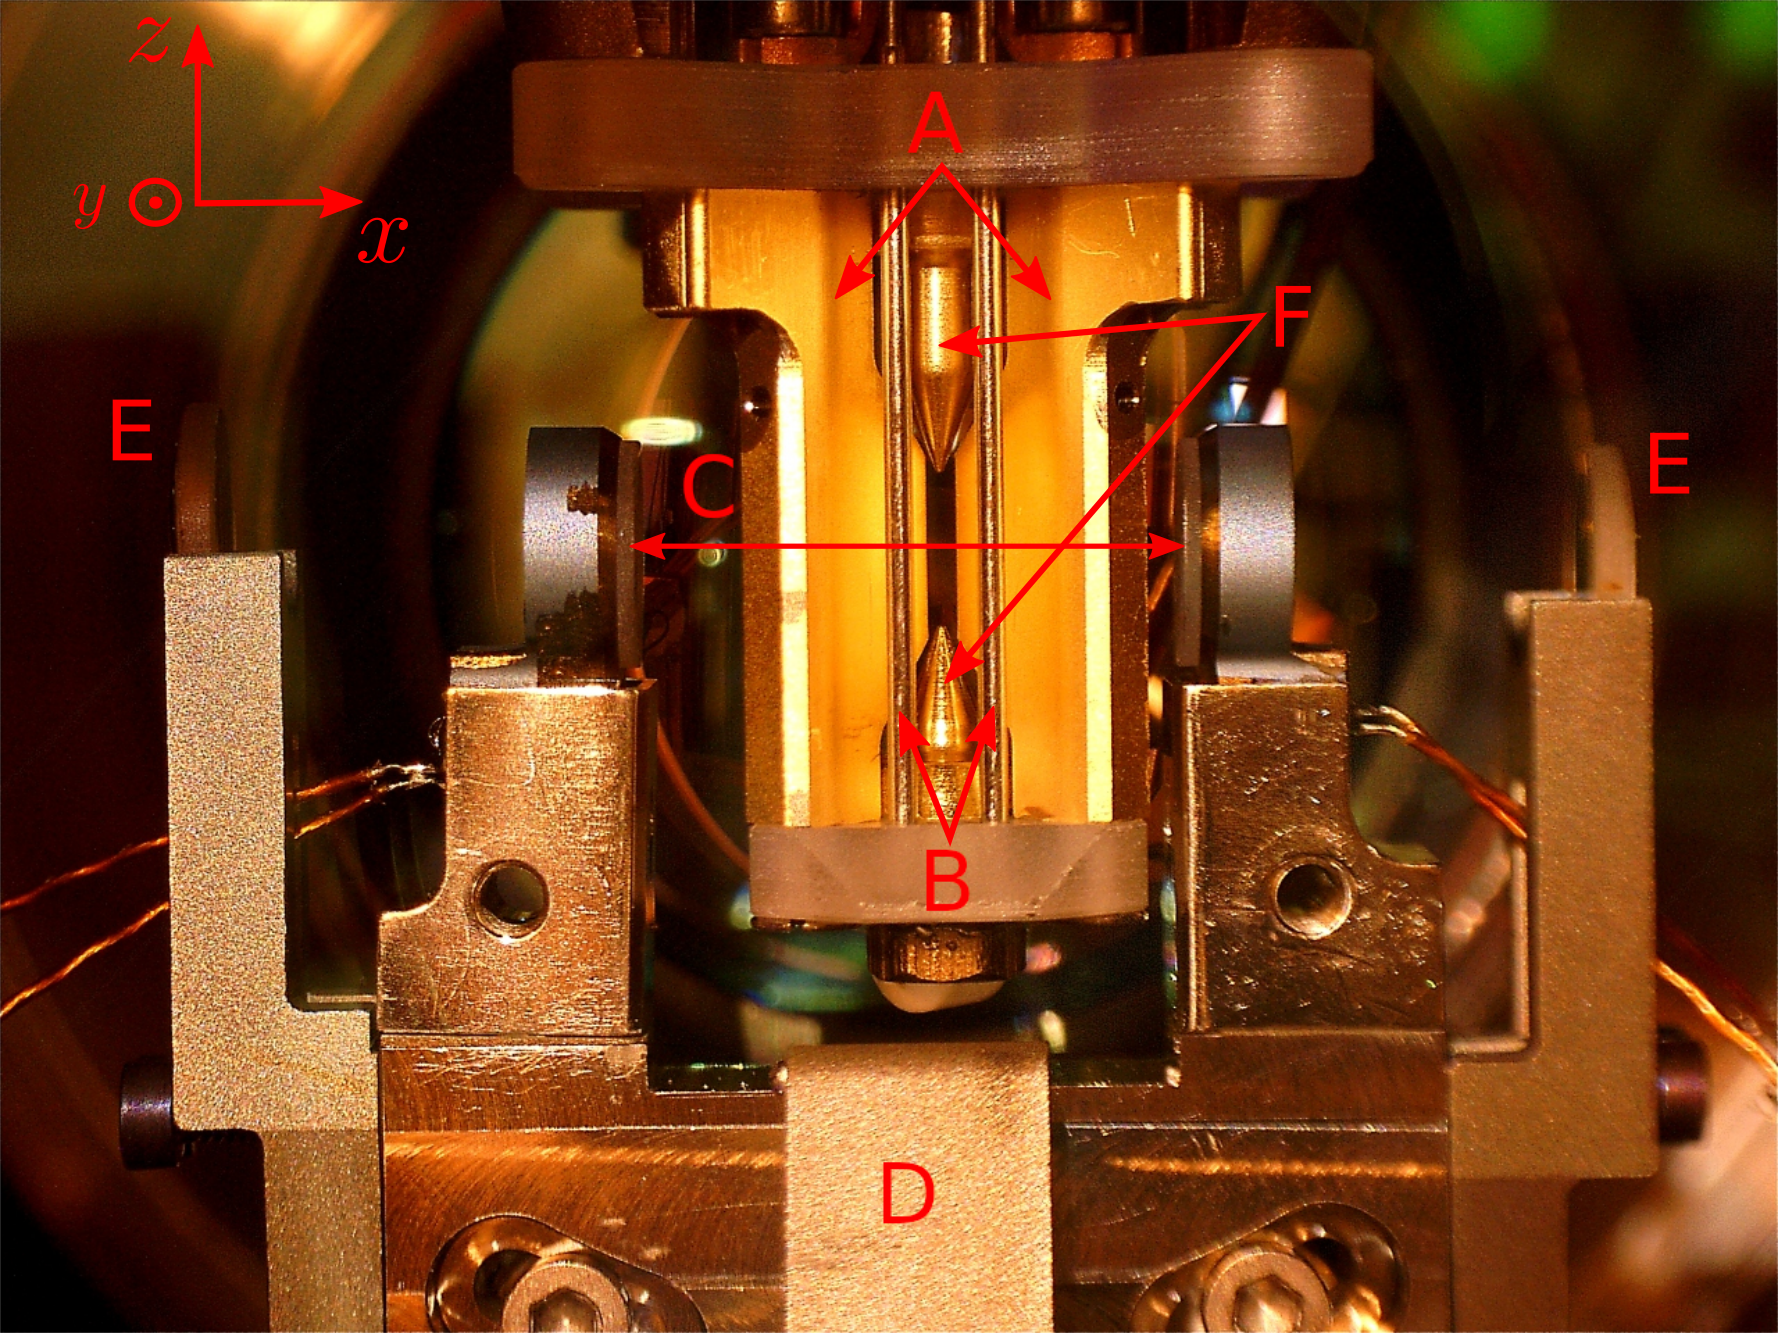
\includegraphics[width = .7\textwidth]{phototrap_withletters_andarrows}
\caption{Photo of the mounted trap. Axial direction is defined along the $z$ axis, while radial is $r^2 = x^2 + y^2$. Highlighted in the image there are: (A) Trap's golden blades for radial RF confinement (B) One pair of compensation electrodes (C) Cavity mirrors, right mirror is highly reflective, left is 854 nm photon output mirror (see section \ref{sec:cavityqed}), separation is $\sim 20$ mm (D) Calcium atomic oven (E) Collimation lenses (F) Static voltage endcaps for axial confinement.}
\label{trapphoto}
\end{figure}
Our trap is a linear 3D RF Paul trap as depicted in figure \ref{trap}, the picture of the real trap is displayed in figure \ref{trapphoto} where main components are highlighted. The electrodes are made in titanium, and are covered in gold. The trap itself is mounted vertically on a Shappire holder. The endcaps are 5 mm apart, and they are usually kept at voltages on the order of 500-1000V, which corresponds to single-ion axial frequencies of $\omega_z \sim 2\pi \times 0.7-1$ MHz respectively. The four blades are 0.8 mm from the center of the trap and driven with an RF of $\sim 24$ MHz. The RF signal from an amplifier is impedance matched with the trap using a quarter-wave bulk helical resonator (not shown). The trap also includes three pairs of compensations electrodes that can be used to compensate for stray electric fields, top view of the trap with compensations electrodes is in figure \ref{clippingtop}.
Loading of ions is done with an atomic oven, calcium is heated and directed towards the trap, where neutral atoms undergo 2-stage photon ionization. One laser 422 nm, resonantly excites one electron to the state 4p$^1\text{P}_1$, while a second laser 375 nm, brings the electron to free space ionizing the atoms \cite{Gulde2001}. Such two stage process allows to filter for isotopes and ionize only $^{40}\text{Ca}$. Loading usually takes minutes or tens of minutes depending on the number of ions one wants to load. Storing time can be in the order of days, especially when a single ion is loaded.\\
Once loaded, ions are Doppler laser cooled with 397 nm light on the transition $\text{S}_{1/2} \to \text{P}_{1/2}$ detuned between $-\Gamma/2$ and resonance\footnote{The choice of cooling closer to resonance is to collect more photons on the camera}. An additional repumper on the transition $\text{P}_{1/2} \to \text{D}_{3/2}$ is also used to avoid the electron being stuck in the $\text{D}_{3/2}$ state. For typical experiments a stage of Doppler cooling is always included, this lasts from 1 millisecond up to tens of milliseconds.\\
With the same Doppler cooling light, imaging can also be done. The light shines on the ions exciting the transition $\text{S}_{1/2} \to \text{P}_{1/2}$ driving the electron to the excited state which then decays spontaneously emitting photons. Photons are collected with a custom objective with NA of $\sim 0.3$, which means an efficiency of 2.5 \% over the solid angle $4\pi$. The objective focuses the collected photons 1.5 meters away where a CCD camera (Andor iXon Ultra 897) is placed. The geometrical path of the imaging is displayed in figure \ref{imgsetup}, this setup has a magnification factor of $\sim$18.6. The same objective is also used for the addressing setup built within this thesis. Therefore, the imaging optical path must be partially shared with the newly built addressing. More details of the objective are given in section \ref{sec:obj}.\\
Consider a qubit encoded in the states $\text{S}_{1/2} \to \text{D}_{5/2}$, if the imaging laser is switched on, the electron will be projected either to the $\text{S}_{1/2}$ level or in the $\text{D}_{5/2} $. In the first case, photons are scattered from the ion and collected on the PMT, in the second case the electron is shelved and will not scatter any photon. Hence, the two cases are distinguishable by counting statistics. A histogram can be constructed  with the number of photon measured, and a properly set threshold differentiates between bright and dark states. Typical detection times are in the order of milliseconds.\\
Laser paths used to perform all of these operations are displayed in figure \ref{imgsetup}.

\begin{figure}
\centering
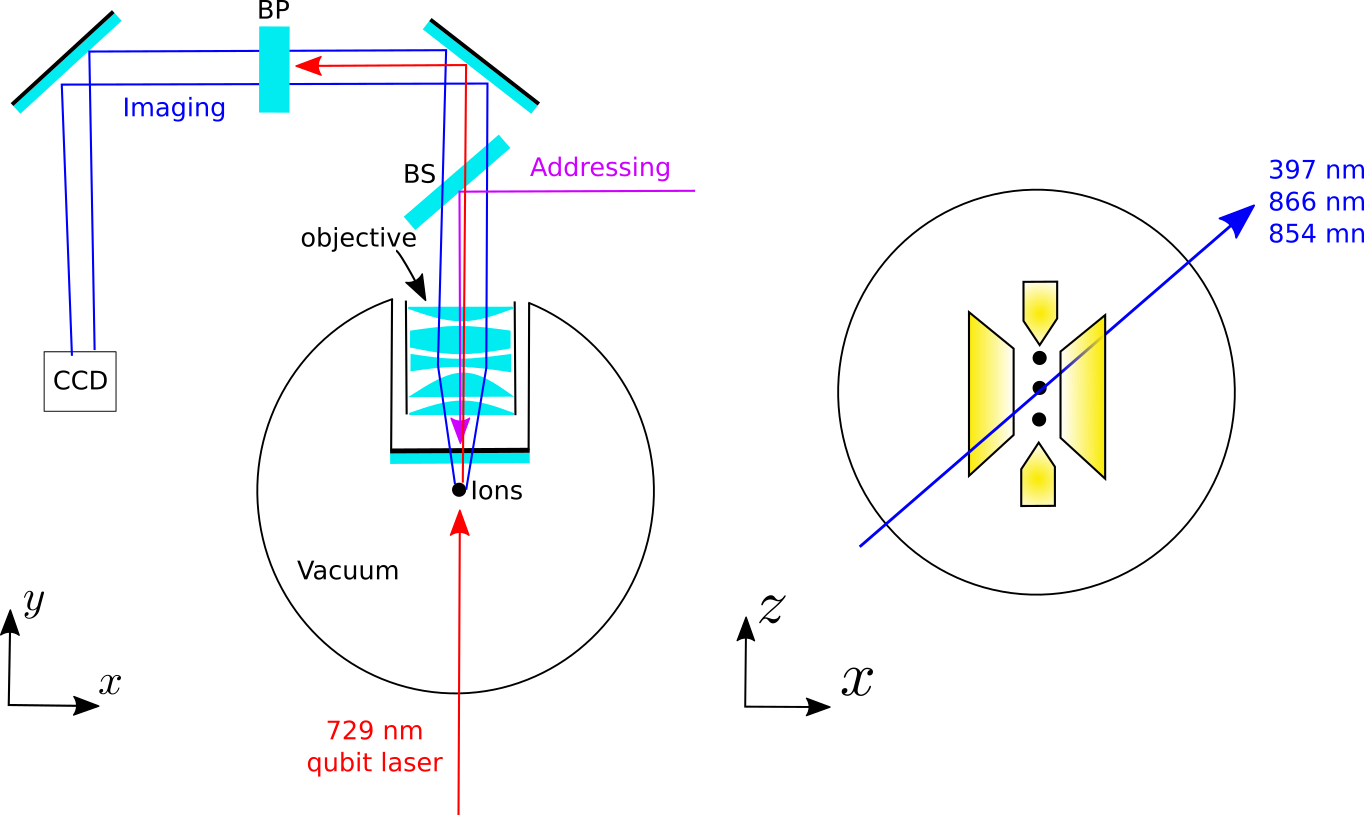
\includegraphics[width = .8\textwidth]{imgsetup}
\caption{Top view of the imaging optical path, the objective collimates and focuses the scatter photons onto the CCD camera. The addressing setup must share part of this path, as the same objective is used for focusing.}
\label{imgsetup}
\end{figure}

\section{393 nm laser}
\begin{figure}[!ht]
\centering
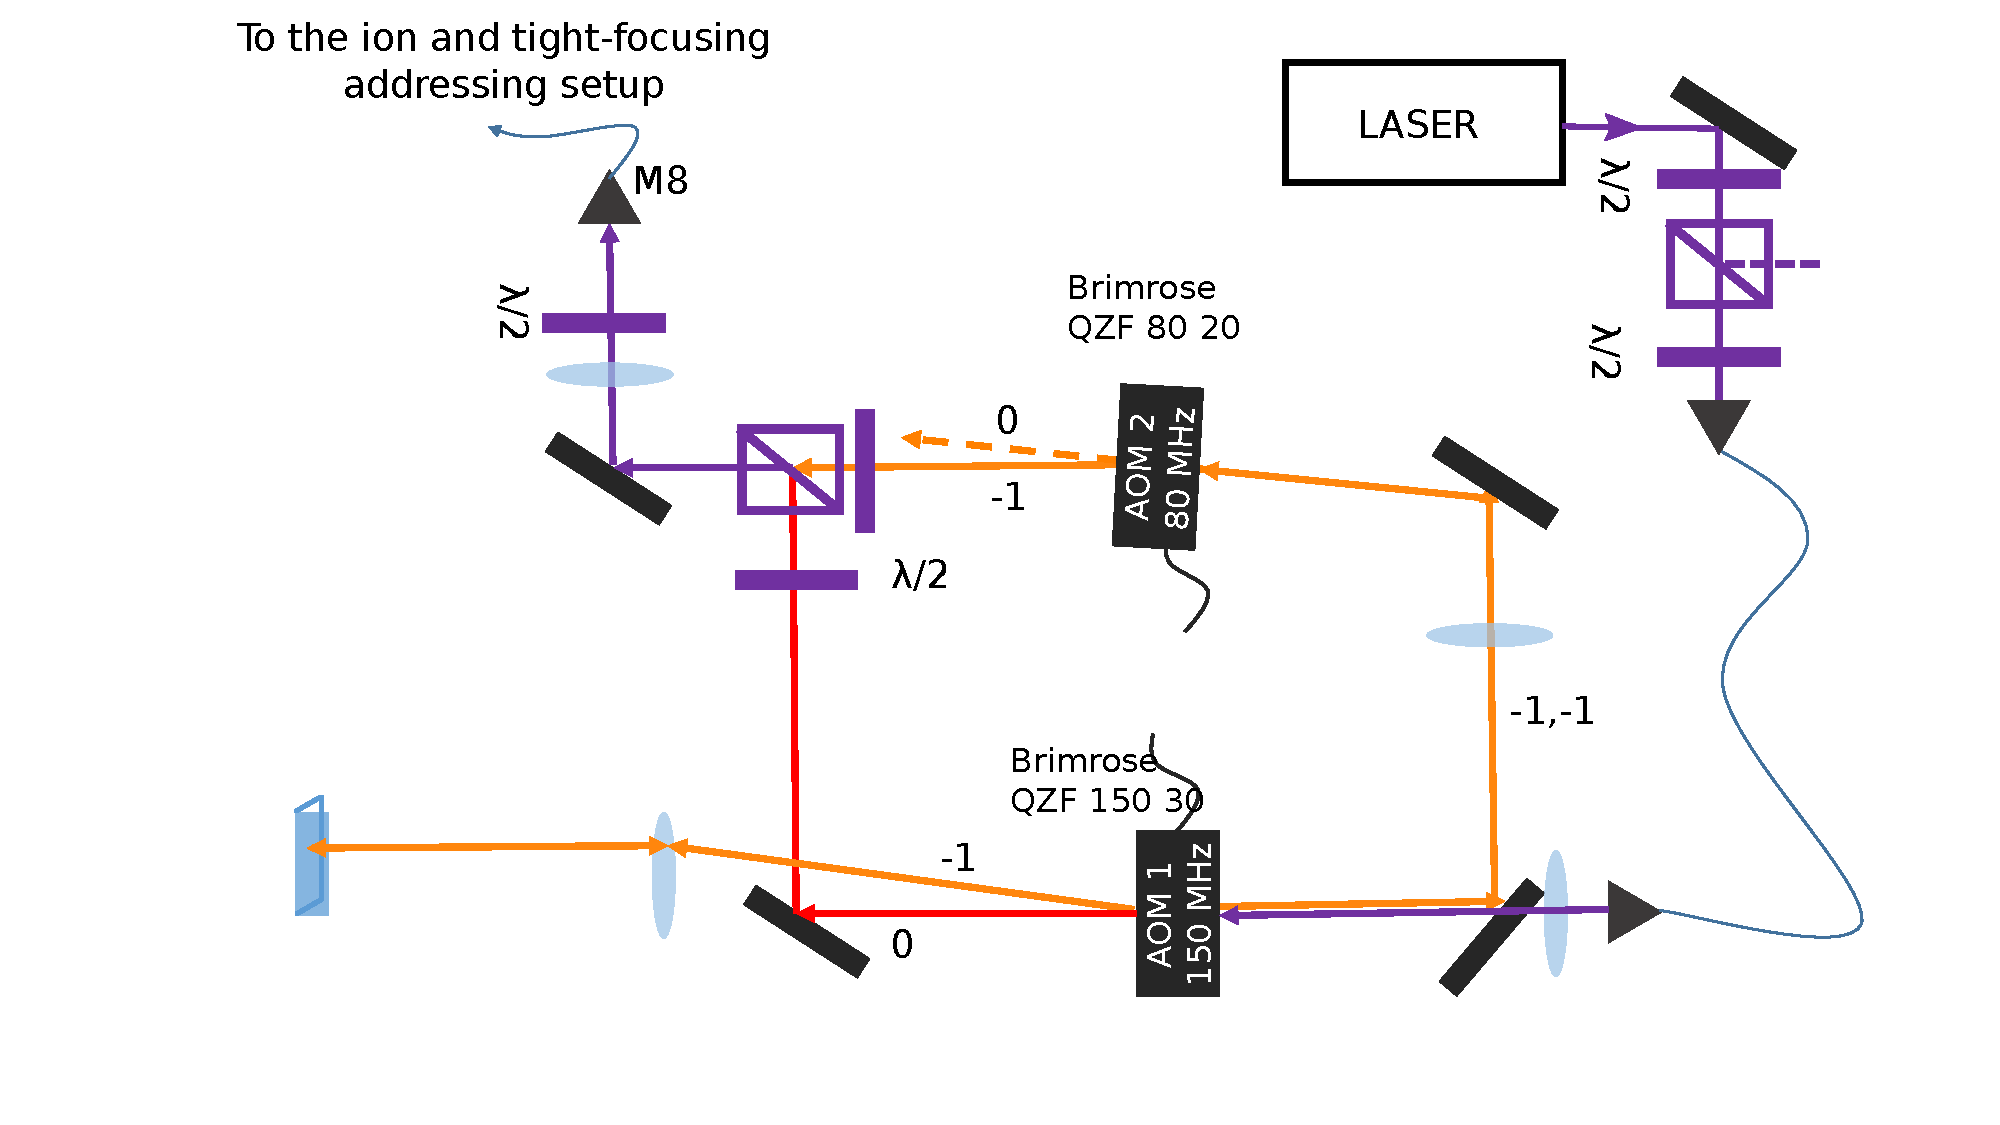
\includegraphics[width = \textwidth]{scheme_393}
\caption{393nm laser optical setup before installing addressing. Two paths are present: a resonant path on the $\text{S}_{1/2} \to \text{P}_{3/2}$ transition (in red), and a detuned path (in orange) where a double pass AOM introduces -300 MHz shift, and a single pass AOM an additional -80 MHz. Paths are overlapped on a beam splitter and coupled to a fiber. Numbers on the paths indicate diffraction order, above the AOM's, model, central frequencies and bandwidths are displayed. Lenses in the setup focus the waist of the beam in the AOM's aperture avoiding unwanted beam steering and therefore losing coupling to the fiber. Setup built by V. Krutianskii, image made by him and adapted for this thesis.
}
\label{scheme393}
\end{figure}
The laser used to drive the Raman transition is 393 nm. This light is obtained from a titanium-sapphire laser from MSquared. The laser is optically pumped with 8 W of light at 532 nm coming from a Lighthouse Photonics Sprout laser. The Ti:Sa crystal is contained in a cavity in a bow tie configuration, together with an optical diode, etalon, birefringent mirror, and tunable cavity mirror for frequency tuning and stabilization. The laser can be frequency locked to a wavemeter or to an external cavity.\\ The fundamental mode is at 786 nm with tunability ranging from 725 nm to 875 nm that can be controlled remotely on the computer. The fundamental light is frequency doubled to 393 nm via a MSquared ECD-X external cavity resonant doubler accessory module. Blue light can be obtained with up to 1 W of power. Before reaching the ion trap, 393 nm light is sent through the setup in figure \ref{scheme393}. The laser serves different purposes, in this thesis it has been used for qubit manipulation as described in section \ref{sec:expqubit}, and for photon generation section \ref{sec:expphoton}. Therefore for flexibility, the setup contains two paths: a resonant with the $\text{S}_{1/2} \to \text{P}_{3/2}$ transition, which goes directly to the ion; and a second path, where the light is detuned by -380 MHz, ideal for exciting the Raman transition described in section \ref{sec:ramanprocess}.\\
The introduction of an AOD in the addressing setup further shifts the light by -125 MHz, as we want to work around -400 MHz to excite the Raman transition,
this setup had to be altered. AOM 2 was switched from -1 order to +1 order, and driving frequencies were changed to 180 MHz for AOM 1 and 70 MHz for AOM 2.

\section{Experiment control}
Complex trapped-ion experiments require control over a large network of AOM's and other devices. Furthermore, precise control over laser phase is also fundamental in some experiments. The need of fast and coherent pulse control is fulfilled by an electronic system that can be controlled with a software on a computer where every device connected to the network can be controlled. The experiment control network is sketched in figure \ref{expcontrol}. The main components are:
\begin{itemize}
\item A computer: from here the experiment is controlled with TrICS (Trapped Ion Control Software)\footnote{A custom software developed internally in the Blatt's group of the University of Innsbruck used for controlling experiments based on trapped ions}.
\item Bus system\footnote{Designed in Innsbruck by G. Hendl.}: parallel communication system between the computer and various electronics such as Direct Digital Synthesizers (DDS).
\item Pulse box: it contains a FPGA and DDSs, it receive experiment sequences from the computer and generates accordingly coherent pulses for the experiment electronics.
\end{itemize}
The computer is connected to the Bus system with a NIDAQ card. DDS used to generate radio frequency signal for AOMs are connected to the Bus system through an optocoupler to avoid ground loops. The computer is connected via Ethernet and with a NIDAQ card to the Pulse Box. The card sends and receive trigger signals, while over the ethernet, experiment sequences are uploaded to the Pulse box.\\
DDSs are present both in the Bus system and in the Pulse box, the difference lies in the fact that DDSs on the Bus system can be controlled on the $\mu$s scale,

 The pulse box contains DDS and and FPGA, thus it has the capabilities of generating short and coherent TTL pulses ($\mu$s) that can send to TTL switches placed between a DDS, the source of the signal, and an AOM. The Pulse Box contains fast switching DDS, this means that the frequency of such DDS can be changed quickly, unlike the DDS on the Bus.\\
With this system, a laser pulse can be controlled in frequency, amplitude, and length. Frequency and amplitude are set in the DDS by sending a signal over the Bus system to th appropriate DDS channel. The length of the pulse can be controlled precisely by the Pulse Box. Moreover, the Pulse Box also has pulse shaping possibilities.\\
In a typical experiment, a sequence of pulses is programmed in python on the computer. When the experiment is run, the computer uploads the sequence to the FPGA inside the Pulse Box. Next, the computer updates the DDSs on the Bus with the appropriate values for the experiment, sends a trigger signal to the Pulse Box and the Pulse Box generates and sends all the signals for the sequence. When the experiment is done, the Pulse box sends another trigger back to the computer, which proceeds to prepare for the next measurement point, it updates the values of the Bus DDS, reupload the code to the Pulse Box, sends a trigger to start the sequence and the loop is repeated.

\begin{figure}
\centering
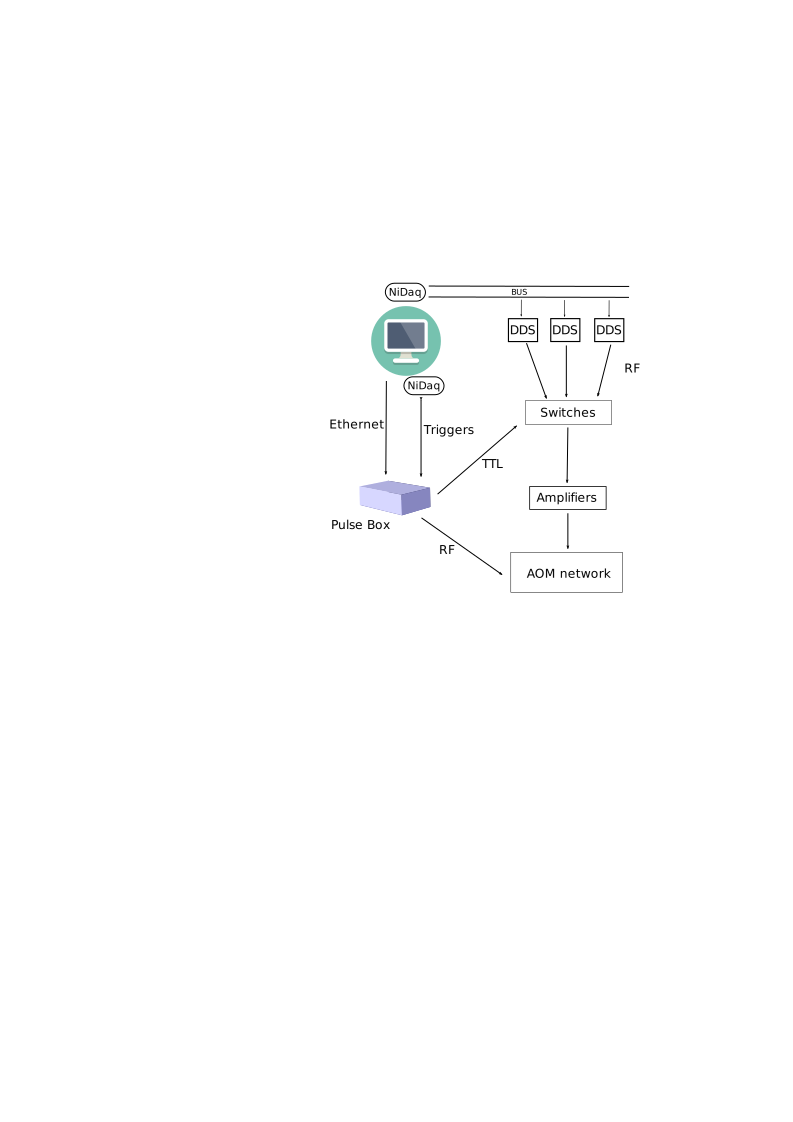
\includegraphics[width =.5\textwidth]{expcontrol}
\caption{Schematic of the experimental control. Everything is controlled remotely by a pc. During a sequence a pulse box generated coherent pulses to the appropriate devices.}
\label{expcontrol}
\end{figure}

\begin{figure}
\centering
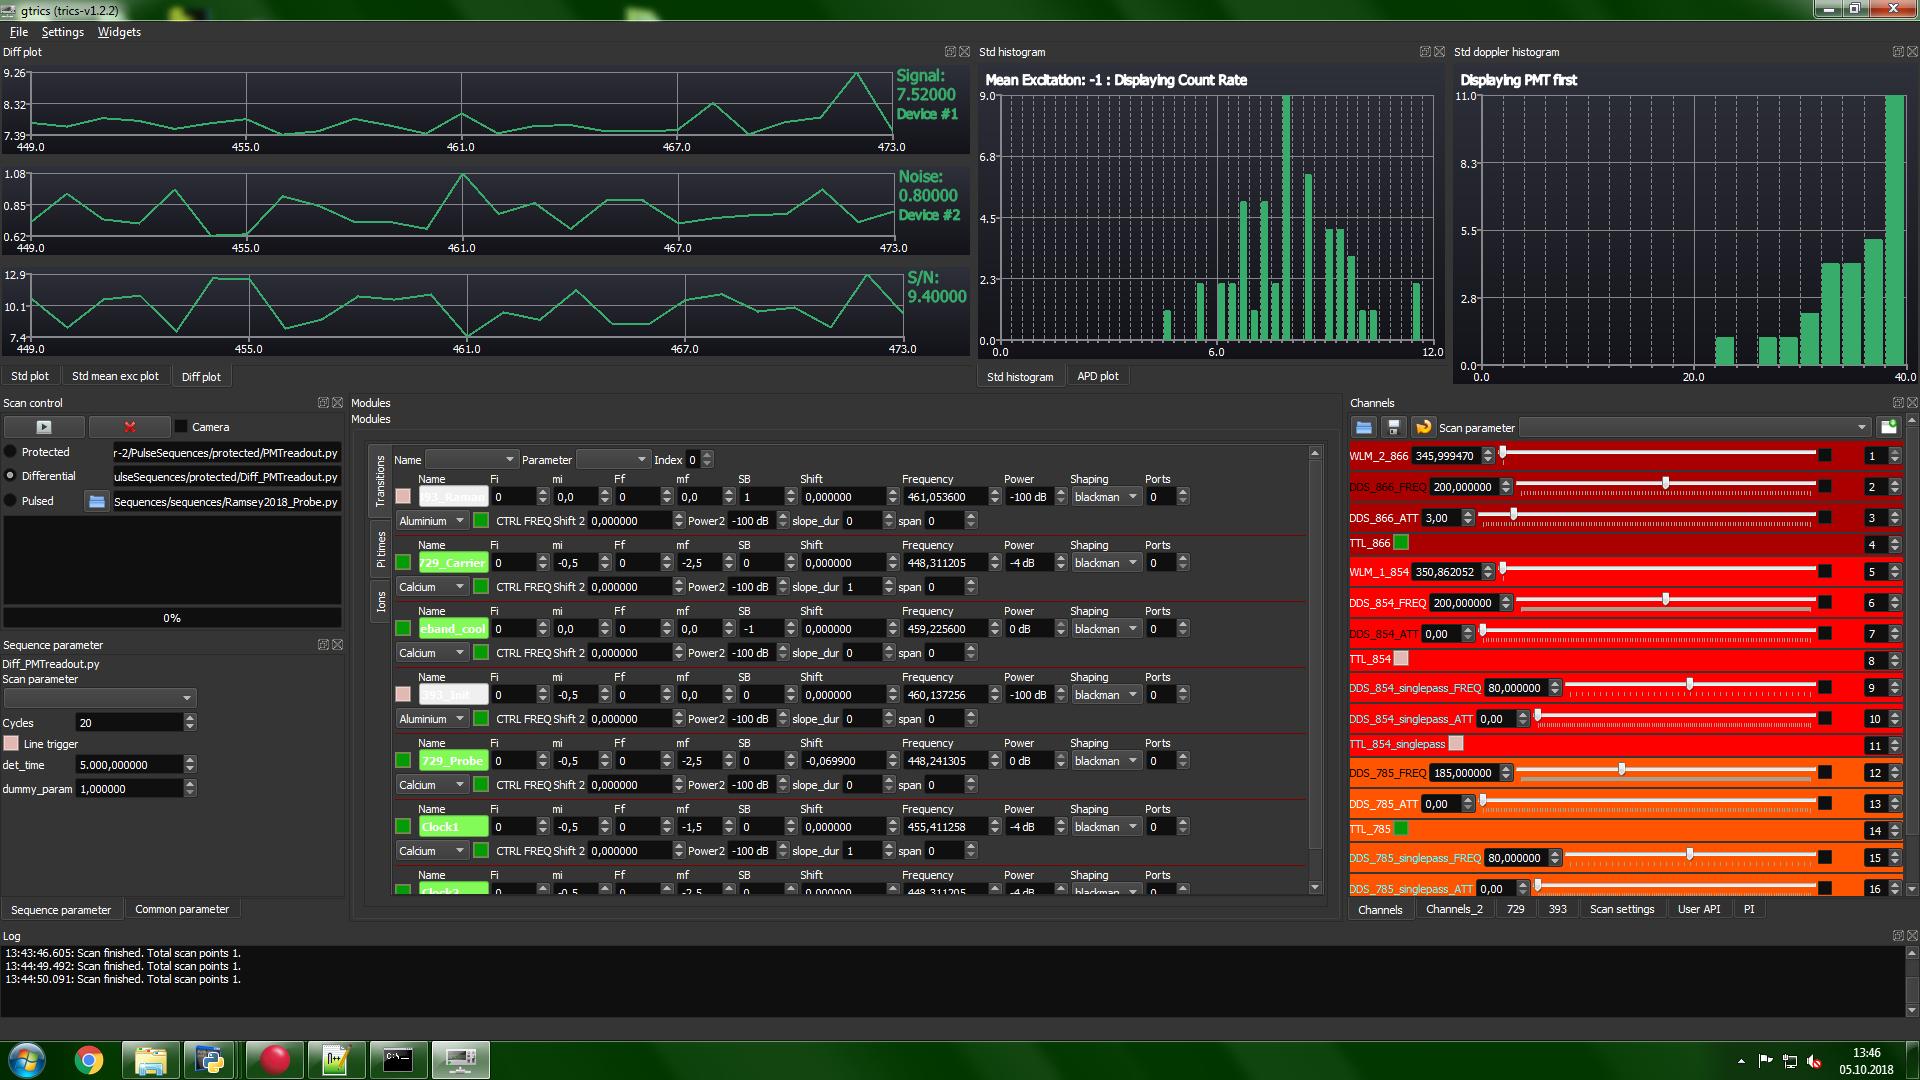
\includegraphics[width =\textwidth]{trics}
\caption{Trics software used to change all the experiment parameters and launch measurements.}
\label{trics}
\end{figure}
